\documentclass{beamer}

\usepackage{array}
\usepackage[english]{babel}
\usepackage[utf8x]{inputenc}
\usepackage{amssymb}
\usepackage{amsmath}
\usepackage{geometry}
\usepackage{graphicx}
\usepackage{eucal}
\usepackage{wrapfig}
\usepackage{datetime}
\usepackage{soul}
\usepackage[font=small,labelfont=bf]{caption}
\usepackage[backend=biber, style=ieee]{biblatex}

\graphicspath{ {./fig} }

\title{Public key cryptography + concept of secure messaging}
\subtitle{Basic abstract algebra with SageMath (cnt.)}
\author{Alexander Buchnev}

\newdateformat{monthYear}{\monthname[\THEMONTH] \THEYEAR}
\date{\monthYear\today}

\addbibresource{./refs.bib}

\DeclareCaptionFormat{custom}
{%
    \textbf{\tiny #1#2}\textit{\tiny #3}
}
\captionsetup{format=custom}

\begin{document}

\frame{
	\titlepage
}

\newtheorem{prop}{Proposition}

%% Proof for the homework

\begin{frame}{Outline}
    \section{Outline}
	\tableofcontents
\end{frame}

\begin{frame}{New directions in cryptography}
    \section{New directions in cryptography}
    In their groundbreaking article \cite{diffie-hellman:1976}, Diffie and Hellman propose new concepts and techniques
    of secure messaging that are still in use (article dates back to 1976!!).
\end{frame}

\begin{frame}{A method for obtaining digital signatures and public-key cryptosystems}
    \section{A method for obtaining digital signatures and public-key cryptosystems}
    A year later, Ronald Rivest, Adi Shamir and Leonard Adleman publish a paper \cite{rsa-1978}, which describes the algorithm, that
	later received name ``RSA''. The proposed method for obtaining public-key cryptosystems is based on underlying problem of integer
    factorisation. For now, there is no evidence that the RSA cryptosystem is prone to polynomial-time attacks running on classical
    computers.
\end{frame}

\begin{frame}{Perfect secrecy}
	\section{Perfect secrecy}
    \begin{wrapfigure}{R}{0.5\textwidth}
        \begin{center}
        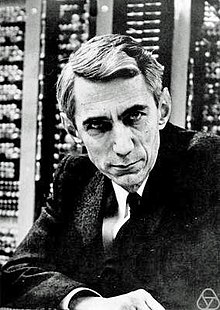
\includegraphics[height=0.35\textheight]{shannon.jpg}
        \end{center}
    \caption{Claude Shannon \\ (source: \href{https://wikipedia.org}{wikipedia.org})}
    \end{wrapfigure}
    In 1948, he published the article `A Mathematical Theory of Communication' \cite{shannon-1948}, where he introduces the notion of entropy as a measure
    of information content in a message. The higher the entropy, the higher the uncertainty of the next symbol in the message and vice
    versa.
\end{frame}

\begin{frame}{Entropy}
    \subsection{Entropy}
    As it was said earlier, entropy is the measure of the information content. Claude Shannon defines entropy in the following way:
    \begin{equation}
        H(\chi) = \sum_{x \in \chi}{p(x) \log p(x) = \mathbb{E}(- \log p(\chi))}
    \end{equation}
\end{frame}

\begin{frame}[shrink=30]{References}
	\section*{References}
    \printbibliography
\end{frame}

\end{document}
